\documentclass[11pt, oneside]{article}   	% use "amsart" instead of "article" for AMSLaTeX format
\usepackage{geometry}                		% See geometry.pdf to learn the layout options. There are lots.
\geometry{letterpaper}                   		% ... or a4paper or a5paper or ... 
%\geometry{landscape}                		% Activate for rotated page geometry
%\usepackage[parfill]{parskip}    		% Activate to begin paragraphs with an empty line rather than an indent

\usepackage{macro}
\usepackage{float}
\usepackage{booktabs}

%SetFonts

%SetFonts

\newcommand{\flow}{\text{flow}}
\newcommand{\bc}{\bar{c}}


\title{Work Plan for Capacity Expansion Model}
\author{Francisco Fonseca}
\date{December 2017}							% Activate to display a given date or no date

\begin{document}
\maketitle
\section{Introduction}

In December 2017, Michael Craig handled the remaining implementation of the RIPS Capacity Expansion (CE) model to me. This document summarizes the work plan for the next steps still needed to be implemented in the code of the model. This list is mostly based on the word document \texttt{RIPSGuide\_Craig\_7Dec17.docx} available in the git repository.

\section{Summary of ``to do' list}

\begin{itemize}
\item Change the source of solar data from NREL Solar Integration Dataset to NSRDB data
\item Update python code to use Aviva's regressions that link capacity deratings (NOT related to regulatory limits) to ambient conditions.
\item If we use Aviva's data, we need to use cell-specific meteorological data from UW.
\item Update demand forecast to include whole SERC (instead of only TVA, which is the current case)
\item Change `specialh' set of hours to include other events (currently it only includes peak demand events)
\item Implement plotting script to draw maps of SERC that shows the output of the model (for example where the plants are being built)
\item Update curtailment procedure to take into account the effect of water temperatures.
\end{itemize}


\section{Details of to do list}

According to Michael, ``[T]he Python code for processing inputs to and outputs from the CE model is largely complete, although some debugging may be necessary.'' He goes on to list some modifications to the model that are pending:

\subsection{Update Solar data source}
Solar data currently comes from the NREL Solar Integration Dataset. However, Bri recommends we instead use NSRDB data, which provides solar irradiance, then use that data to estimate PV generation. I have downloaded NSRDB data at points in a grid over the entire region (Databases/NSRDBRIPS). In the SolarMOEPaper folder, there are Python scripts for inputting NSRDB data to PVLib to get estimated hourly generation. (\texttt{GetRenewableCFs} script)

\subsection{Update use of Aviva's regressions}

Right now, the Python code has placeholder code to insert Aviva's regressions that link capacity deratings (NOT related to regulatory limits) to ambient conditions. You will need to update the form and coefficients in these regressions and the mapping of plants to regressions.  (\texttt{CurtailmentRegressions} script)

\subsection{Read UW meteo data by cell}

The code loads meteorological data at the regional rather than cell-specific data. If you do use regressions from Aviva, you will need to use cell-specific meteorological data from UW.  (\texttt{ModifyGeneratorCapacity} script and \texttt{loadMetData} function)


\subsection{Update demand forecast to whole SERC}

The CE model currently uses Francisco's demand forecast for TVA. That code should be updated for the Southeast when regressions are available. \\ \texttt{ForecastDemandWithRegression}

\subsection{Update 'speciah' set of hours}

The CE model has a ``specialh' set of hours, which is currently used to include hours from the day with peak demand. However, you may also want to include days with peak curtailment of generators. If so, then you will need to add a set of hours for these peak curtailment hours. I did not because the day with peak demand may very well overlap with the day with peak curtailment. (\texttt{DemandFuncsCE} script, \texttt{selectWeeksForExpansion} function (also will require modifications to GAMS code))

\subsection{Update curtailment 1}

Need to finicsh implementing the curtailment equations, which use simple mixing formula, from the CurtailmentEquations.doc document. The environmental regulation equation currently includes water flow (availability), but the availability data is not being loaded in the RIPSMasterScript yet

\begin{itemize}
\item For loading water availability data: \texttt{ModifyGeneratorCapacityWithWaterTData} script and \texttt{loadWaterAndMetData} function
\item For including availability in curtailments: \texttt{CurtailmentFromEnviroRegs} script and \texttt{CurtailmentFromEnviroRegs} function
\end{itemize}

\subsection{Map output}

The result of this model will be the decisions of building different classes of power plants in different regions of the southeast according to demand forecast and climate related constraints. It would be interesting to implement a tool/function in order to be able to visualize these results on a plot. I have not decided what this tool would look like. But one possibility is to have a gridded map (or several gridded maps) where we could observe where the power plants are being installed. I know how to do it in R, but I need to look at how to do it in Python. I have started looking at it, so we can create maps of the output like this.

\begin{figure}[H]
   \centering
   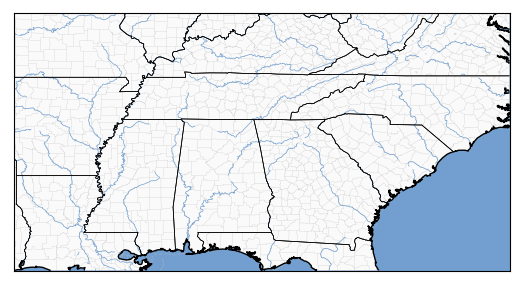
\includegraphics[width=0.8\textwidth]{../../maps/example} % requires the graphicx package
   \caption{example map output}
%   \label{fig:example}
\end{figure}

\subsection{Update curtailment 2}
Paulina mentioned that the curtailment procedure should be also a function of the stream temperatures. As the water temperatures increase, power plants will need to intake a larger amount of water in order to be able to perform the cooling. Right now the amount of water intake is NOT a function of stream temperature. Michael has explicitly defined that the increase in the temperature of the cooling water after it goes through the condenser ($\delta T_g$) is a design parameter of the power plant's condenser that does not depend on the actual stream flow temperature.

One solution would be to use a curve of values for $\delta T_g$ that change with the stream temperature. The way I see it this would not add complexity to the pre processing part. However, one challenge would be to find values for these hypothetical curves. I still don't know if generators have such information available.

\subsection{Low priority: Wind data}

Wind generation data right now comes from the WIND dataset. I chose 2009 generation data because it has a moderate average CF, but you may want to select a different year. If there's a TMY in the WIND data, that would be the best route (you can ask Bri this). 

\subsection{``Tweaks'' and Checks once the model is running}

\begin{itemize}
\item How quickly the CE model runs will partly determine how many days you can include in it. If you include many, then how I currently handle max generation in each set of days by each hydro plant is OK
\item You should revisit special days that are included in the CE model, and think of other possible interesting days to examine. For these days, you?ll have to figure out how you want to set maximum hydropower generation on those days. 
\item I did not observe charging by the pumped hydro units in the CE model. I?m not sure if this is a bug or if there was never a reason for them to, so I would check that later after adding the features above. Like I said, pumped hydro will add significant computational burden, so you may end up eliminating it.
\end{itemize}


\newpage
\section{Capacity Expansion model}

This section presents the formulation of the Capacity Expansion (CE) optimization model. I tried the definitions of variables and equations as close as possible to the way they are defined in the \texttt{.gams} file. This way it should be easier to debug the optimization problem. For example, instead of defining a single variable $n_{(\cdot)}$ for the number of new generators in each pair (location, type), I used the same definitions as the \texttt{.gams} file and created three variables: $n^{(c)}_{c, j}$, $n^{(\bc)}_{z, j}$ and $n^{(r)}_{z, j}$ (which refer, respectively, to thermal generators that can be curtailed, thermal generators that cannot be curtailed and renewable generators).

\subsection{Definitions}

\begin{table}[H]
   \centering
   \caption{Decision Variables}
   \begin{tabular}{p{1in} p{4in} } % Column formatting, @{} suppresses leading/trailing space
      \toprule
      \textbf{Set} & \textbf{Definition} \\
      \midrule
      $n^{(c)}_{c, j}$ & number of new thermal generators of type $j$ in the class that CAN be curtailed (the $(c)$ superscript) built in CELL $c$\\
      $n^{(\bc)}_{z, j}$ & number of new thermal generators of type $j$ in the class that CANNOT be curtailed (the $(\bc)$ superscript) built in ZONE $z$\\
      $n^{(r)}_{z, j}$ & number of new generators of type $j$ in the class RENEWABLE (the $(r)$ superscript) built in ZONE $z$\\
      $p^{(c)}_{c, j, t}$ & electricity generation (GWh) at time $t$ of new generators  of type $j$ in the  class that CAN be curtailed (the $(c)$ superscript) built in CELL $c$\\
      $p^{(\bc)}_{z, j, t}$ & electricity generation (GWh) at time $t$ of new generators of type $j$ in the class that CANNOT be curtailed (the $(\bc)$ superscript) built in ZONE $z$\\
      $p^{(r)}_{z, j, t}$ & electricity generation (GWh) at time $t$ of new generators  of type $j$ in the class RENEWABLE (the $(r)$ superscript) built in ZONE $z$\\
      $p^{(e)}_{i, t}$ & electricity generation (GWh) at time $t$ of existing (the $(e)$ superscript) generator of index $i$ \\
      $\flow_{\ell, t}$ & flow on line $\ell$ (GW) in hour $t$\\
%
      \bottomrule
   \end{tabular}
   \label{tab:decision}
\end{table}

% Requires the booktabs if the memoir class is not being used
\begin{table}[H]
   \centering
   \caption{Sets}
   \begin{tabular}{p{1in} p{4in} } % Column formatting, @{} suppresses leading/trailing space
      \toprule
      \textbf{Set} & \textbf{Definition} \\
      \midrule
      $\Bc$ & set of user-defined time blocks. These are needed for computational purposes. $\Bc = \{\text{peak-hours, winter, summer, spring, fall, special periods}\}$ \\
      $\Ic$ & set of existing generators in the fleet. \\
      $\Ic (z)$ & subset of existing generators that are located in zone $z$.  $\Ic (z) \subseteq \Ic$\\
      $\Cc$ & set of grid cells that new techs can be placed in. \\
      $\Cc (z)$ & subset of grid cells that new techs can be placed in that are located in zone $z$. $\Cc (z) \subseteq \Cc$\\
      $\Jc$ & set of candidate plant types for new construction \\
      $\Jc^{(c)}$ & subset of plant types for new construction that can be curtailed. $\Jc^{(c)} \subseteq \Jc$\\
      $\Jc^{(\bc)}$ & subset of plant types for new construction that CANNOT be curtailed. $\Jc^{(\bc)} \subseteq \Jc$\\
      $\Jc^{(r)}$ & subset of plant types for new construction that are renewable. $\Jc^{(r)} \subseteq \Jc$\\
      $\Lc$ & set with transmission lines between load zones \\
      $\Zc$ & set with user defined load zones \\
      \bottomrule
   \end{tabular}
   \label{tab:sets}
\end{table}


% Requires the booktabs if the memoir class is not being used
\begin{table}[H]
   \centering
   \caption{Parameters}
   \begin{tabular}{p{1in} p{4in} } % Column formatting, @{} suppresses leading/trailing space
      \toprule
      \textbf{Parameter} & \textbf{Definition} \\
      \midrule
      $P^{MAX}_{c, j, t}$ & Maximum electricity generation capacity, accounting for deratings, of plant type $j \in \Jc^{(c)}$ at cell grid $c$ at time $t$ (MWh) \\
      $P^{NP}_{j}$ & Nameplate electricity generation capacity of plant type $j \in \Jc$ (MWh)\\
      $P^{MAX}_{i, t}$ & Maximum electricity generation capacity, accounting for deratings, of existing generator $i$ (non solar and non wind) at time $t$ (MWh)\\
      $P^{MAX}_{solar, t}$ & Maximum electricity generation by all existing solar generators at time $t$ (MWh) \\
      $P^{MAX}_{wind, t}$ & Maximum electricity generation by all existing wind generators at time $t$ (MWh) \\
      $\overline{\flow}_{\ell}$ &  Upper bound of transmission line $\ell$ (GW)\\
      $FOM_{j}$ & Annual fixed operation and maintenance costs of plant type $j$ (\$/MW)\\
      $OCC_{j}$ & Overnight capital cost of plant type $j$ (\$/MW) \\
      $OC_{j}$ & Operating cost of plant type $j$\ (\$/MWh) \\      
      $OC_{i}$ & Operating cost of existing plant $i$\ (\$/MWh) \\
      $M$ & Planning reserve margin as fraction (\%) of demand \\
      $Q$ & Discount rate \\
      $D_j$ & lifetime (years) of candidate plant of type $j$ \\
%      
      \bottomrule
   \end{tabular}
   \label{tab:indices}
\end{table}


% Requires the booktabs if the memoir class is not being used
\begin{table}[H]
   \centering
   \caption{Indices}
   \begin{tabular}{p{1in} p{4in} } % Column formatting, @{} suppresses leading/trailing space
      \toprule
      \textbf{Indices} & \textbf{Definition} \\
      \midrule
      $b$ & Time blocks representing peak-hours, winter, summer, spring, fall, special periods. $b \in \Bc$\\
      $c$ & grid cells that new techs can be placed in. $c \in \Cc$ \\
      $\ell$ & Transmission Lines. $\ell \in \Lc$\\
      $i$ & existing generators in fleet. $i \in \Ic$\\
      $z$ & sub regions of SERC. $z \in \Zc$\\
      \bottomrule
   \end{tabular}
   \label{tab:indices}
\end{table}

\subsection{Objective Function}

\begin{equation} \label{eq:obj_fun}
\begin{split}
TC = &  \sum_{c \in \Cc}\sum_{j \in \Jc^{(c)}} n^{(c)}_{c, j} \times P^{NP}_{j} \times (FOM_{j} + OCC_{j} \times CRF_{j}) \\
& +  \sum_{z \in \Zc}\sum_{j \in \Jc^{(\bc)}} n^{(\bc)}_{z, j} \times P^{NP}_{j} \times (FOM_{j} + OCC_{j} \times CRF_{j}) \\
& +  \sum_{z \in \Zc}\sum_{j \in \Jc^{(r)}} n^{(r)}_{z, j} \times P^{NP}_{j} \times (FOM_{j} + OCC_{j} \times CRF_{j}) \\
& + \sum_b \bigg( W_b \sum_{t_b \in T_b}\bigg( \sum_{c \in \Cc}\sum_{j \in \Jc^{(c)}} p^{(c)}_{c, j, t_b} \times OC_{j, t_b} + \sum_{z \in \Zc}\sum_{j \in \Jc^{(\bc)}} p^{(\bc)}_{z, j, t} \times OC_{j, t_b} \\
& \qquad\qquad\qquad\qquad +  \sum_{z \in \Zc}\sum_{j \in \Jc^{(r)}} p^{(r)}_{z, j, t_b} \times OC_{j, t_b} + \sum_{i} p_{i, t_b} \times OC_{i, t_b} \bigg)\bigg)
\end{split}
\end{equation}

$CRF_j$ is the capital recovery ratio of each technology $j$ and is defined as:

\begin{equation} \label{eq:cap_rec}
\begin{aligned}
CRF_j = \frac{Q}{1-\left(1/(1+Q)^{D_j}\right)}
\end{aligned}
\end{equation}

The variable operating cost $OC$ (in \$/MWh) for new and existing generators is equal:

\begin{align} \label{eq:oc}
OC_{j} = VOM_{j} + HR_{j} \times FC_{j}  &&  \forall~j \in \Jc && \text{(new generators)}\\
OC_{i} = VOM_{i} + HR_{i} \times FC_{i}  && \forall~i \in \Ic && \text{(existing generators)}
\end{align}

NOTE: I followed the same convention as the GAMS code, where the operating cost $OC$ does not change by time $t$ or location $c$.

\subsection{Supply vs Demand constraint}

\begin{equation} \label{eq:supply_demand}
\begin{split}
P^D_{t, z} = & \sum_{i \in \Ic(z)} p_{i, t} +  \sum_{c \in \Cc (z)}  \sum_{j \in \Jc^{(c)}} p^{(c)}_{c, j, t_b} + \sum_{j \in \Jc^{(\bc)}} p^{(\bc)}_{z, j, t_b} +  \sum_{j \in \Jc^{(r)}} p^{(r)}_{z, j, t_b} \\
& +  \sum_{\ell: \text{end}(\ell) = z} \flow_{\ell, t} - \sum_{\ell: \text{begin}(\ell) = z} \flow_{\ell, t}
\end{split}
\end{equation}

\subsection{Reserve margin constraint}

\begin{equation} \label{eq:reserve}
\begin{split}
(1+M)\times P^D_{t, z} \le & \sum_{c \in \Cc} \sum_{j \in \Jc^{(c)}} P^{MAX}_{c, j, t} \times n^{(c)}_{c, j} +   \sum_{j \in \Jc^{(r)}} P^{MAX}_{z, j, t} \times n^{(r)}_{z, j}\times CF_{j, t} \\
& + \sum_{i \in \Ic \setminus \{\Ic_w \cup \Ic_s \}} P^{MAX}_{i, t} + P^{MAX}_{\text{solar}, t} + P^{MAX}_{\text{wind}, t}
\end{split}
\end{equation}

\subsection{Maximum generation constraints}

\begin{equation} \label{eq:ex_solar}
\begin{split}
\sum_{i \in \Ic_s} p_{i, t} \le P^{MAX}_{\text{solar}, t} \quad \forall~t
\end{split}
\end{equation}

\begin{equation} \label{eq:ex_wind}
\begin{split}
\sum_{i \in \Ic_w} p_{i, t} \le P^{MAX}_{\text{wind}, t} \quad \forall~t
\end{split}
\end{equation}

\begin{equation} \label{eq:ex_therm}
\begin{split}
p_{i, t} \le P^{MAX}_{i, t} \quad \forall~t, \forall~i \in \Ic \setminus \{\Ic_w \cup \Ic_s \}
\end{split}
\end{equation}

\begin{equation} \label{eq:new_therm}
\begin{split}
p^{(c)}_{c, j, t} \le P^{MAX}_{c, j, t} \times n^{(c)}_{c, j} \quad \forall~c, t  \text{ and }\forall~j\in \Jc^{(c)}
\end{split}
\end{equation}

\begin{equation} \label{eq:new_therm2}
\begin{split}
p^{(\bc)}_{z, j, t} \le P^{MAX}_{z, j, t} \times n^{(\bc)}_{z, j} \quad \forall~z, t  \text{ and }\forall~j\in \Jc^{(\bc)}
\end{split}
\end{equation}

\begin{equation} \label{eq:new_ren}
\begin{split}
p^{(r)}_{z, j, t} \le n^{(r)}_{z, j}\times P^{NP}_{j} \times CF_{j, t}  \quad \forall~z, t  \text{ and }\forall~j\in \Jc^{(r)}
\end{split}
\end{equation}

\subsection{Transmission Constraint}

\begin{equation} \label{eq:trans}
\begin{split}
0 \le \flow_{\ell, t} \le   \overline{\flow}_{\ell} \quad \forall~\ell, t
\end{split}
\end{equation}


\newpage
\section{Curtailment Equations}

Michael implemented a method to simulate power plant curtailments for sites equipped with once-through cooling due to \underline{REGULATORY LIMITS}. It uses two equations --  a thermal mixing equation and a power plant discharge equation -- to capture the enforcement of environmental regulations.

\subsection{Previous work}

Van Vliet et al did a study to estimate curtailments for power plants with once-through cooling due to environmental regulations. However their equations applied the constraints on the temperature of the power plant discharge and not on the final stream temperature after the mixing has occurred. Therefore, the curtailment constraints end up being stronger. 

\begin{equation}
q = \text{KW}\cdot\frac{1-\eta_{total}}{\eta_{elec}}\cdot\frac{(1-\alpha)}{\rho_w\cdot C_p\cdot\max{(\min{(Tl_{max} - T_w, \Delta Tl_{max})}, 0)}}
\end{equation}

\begin{equation}
\text{KW}_{max} = \frac{\min{(\gamma\cdot Q, q)} \cdot \rho_w\cdot C_p\cdot\max{(\min{(Tl_{max} - T_w, \Delta Tl_{max})}, 0)}}{\frac{1-\eta_{total}}{\eta_{elec}}\cdot \lambda \cdot(1-\alpha)}
\end{equation}

where $\lambda, \eta_{total}, \eta_{elec}, \rho_w, C_p, \alpha, \gamma$ are constants; KW is installed capacity; $q$ is water withdrawal and discharge by a power plant; $Tl_{max}$ and $ \Delta Tl_{max}$ are regulatory stream temperature limits (respectively, actual temperature and increase in stream temperatures) ; $\text{KW}_{max}$ is the maximum achievable capacity; and $T_w$ is the simulated daily water temperature at the power plant location. 

However, the regulatory limits should be applied to the final river temperature.

\subsection{New approach}

Michael's new approach will apply the regulatory constraints over the stream temperature after the mixing, which is how they are supposed to be applied.

The first equation is a thermal balance equation, that computes the final stream temperature after the mixing of the water from the river and the heated discharge from the power plant occur:

\begin{equation}
T_x = \frac{\frac{m_g}{m_r}T_g + T_r}{\frac{m_g}{m_r} + 1} = T_r + \frac{\frac{m_g}{m_r}}{\frac{m_g}{m_r} + 1}\cdot \Delta T_g = T_r + \frac{m_g}{m_g + m_r}\cdot \Delta T_g
\end{equation}

where $T_x$ is the mixed stream temperature; $m_g$ is the flow of the power plant discharge; $m_r$ is the upstream flow of the river; $T_r$ is the upstream stream temperature (before mixing), or stream temperature in that cell; $T_g$ is the temperature of the power plant discharge, which equals $T_r + \Delta T_g$; and $\Delta T_g$ is the increase in temperature of cooling water through the condenser, which we assume is a fixed value that depends on condenser design. 

The second equation is similar to the first from van Vliet. It estimates the withdrawal/discharge flow from a power plant by using the value of $\Delta T_g$ as a design variable at the condenser.

\begin{equation}
m_g = \min{\left (\gamma \cdot m_r, p \cdot \frac{1-\eta - k_{os}}{\eta} \cdot \frac{1}{\rho_w \cdot C_p \cdot \Delta T_{g}}\right)}
\end{equation}

where $\eta$ is the net plant efficiency, which equals 3.412 divided by the plant net heat rate; $k_{os}$ is the fraction of waste heat lost to other heat sinks, which equals 12\% for coal-fired plants and 20\% for gas-fired plants per Bartos and Chester; $p$ is the power output of the power plant; and $\gamma$ indicates the maximum fraction of the river flow that can be extracted for cooling purposes. 

Combining the two equations, we get:

\begin{equation}
T_x = T_r + \left( \frac{ \min{\left (\gamma \cdot m_r, p \cdot \frac{1-\eta - k_{os}}{\eta} \cdot \frac{1}{\rho_w \cdot C_p \cdot \Delta T_{g}}\right)}}{ \min{\left (\gamma \cdot m_r, p \cdot \frac{1-\eta - k_{os}}{\eta} \cdot \frac{1}{\rho_w \cdot C_p \cdot \Delta T_{g}}\right)} + m_r}\right)\cdot \Delta T_g
\end{equation}

Our objective is to find the maximum value of $p$ such that $T_x$ is still less than the environmental limit. However, we can't analytically solve the above equation for $p$ . Also, it does not explicitly account for environmental limits. However, given a mixed stream temperature $T_x$, I can compare that to the regulatory limit and determine whether the power plant needs to be curtailed. 

Specifically, for each power plant, I can test a range of power output values between 0 and its maximum capacity and determine the maximum potential power output before mixed stream temperatures exceed regulatory limits (this would be performed in the pre-processing phase). The same approach can be applied in conjunction with the upriver stream temperature to capture regulatory limits on the change in water temperatures.

One current issue with this approach is that we simplify it by assuming that $\Delta T_g$ is a fixed design parameter of the power plant condenser. However, the actual temperature change through the  condenser may depend on external variables such as water temperature ($T_r$). That is, on very hot summer days, the condenser may not be able to achieve its designed temperature change, requiring a greater intake. One possible solution would be to parametrize the value of $\Delta T_g$ as a function of $T_r$. 

\end{document}  